%UNIT 13: SECOND ORDER LINEAR DEs
%%%%%%%%%%%%%%%%%%%%%%%%%%%
%%%% Put the following at the top of each .tex file  %
\pagestyle{fancy}
\renewcommand{\theUnit}{4.3}
\ifthenelse{\isundefined{\UnitPageNumbers}}{}{\setcounter{page}{1}}
\rhead{Section \theUnit: Homogeneous Second Order Linear DEs}
\lhead{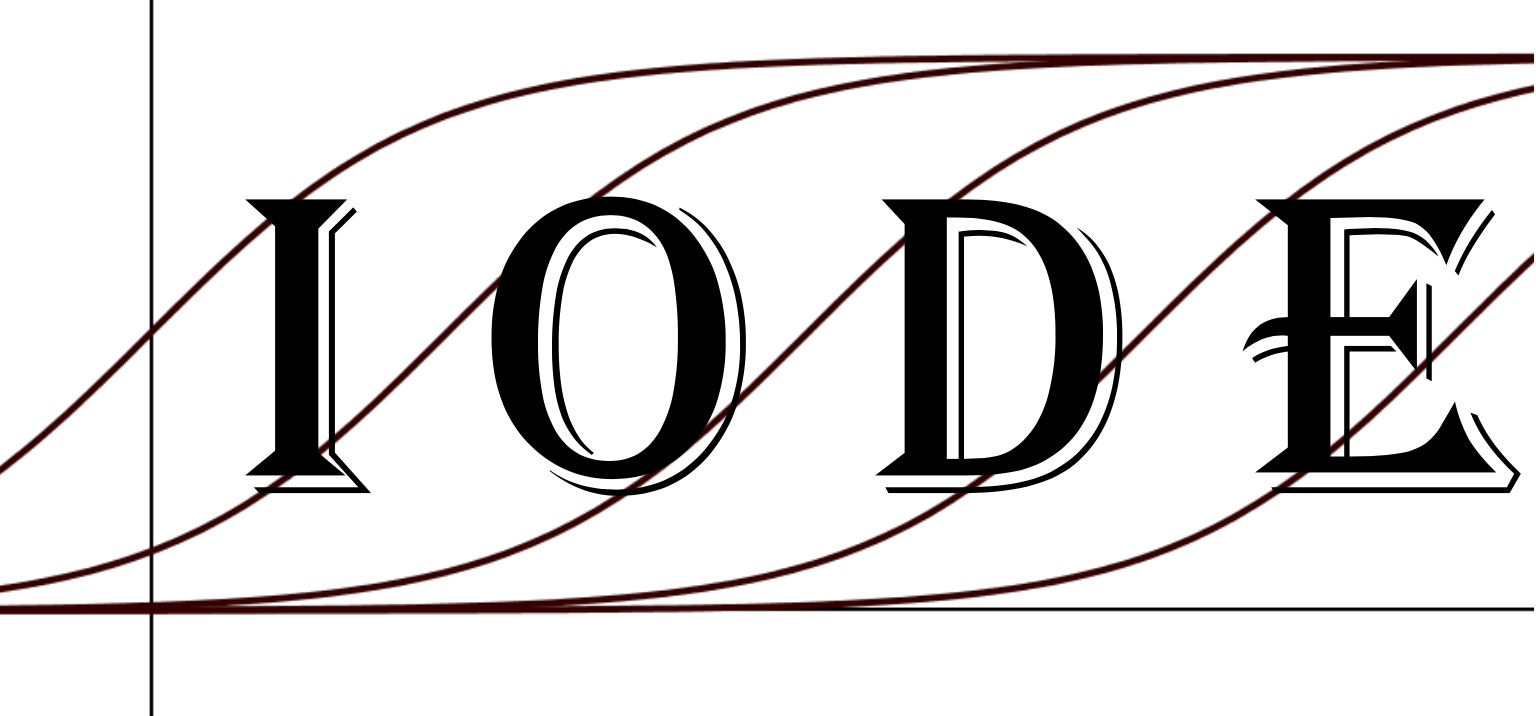
\includegraphics[width=1.25cm]{IODE-logo.png}}
\rfoot{\mypage}
\lfoot{}
\cfoot{}
\fancypagestyle{firstfooter}{\footskip = 50pt}
\renewcommand{\footrulewidth}{.4pt}
%%%%%%%%%%%%%%%%%%%%%%%%%%%
\vspace*{-20pt} \thispagestyle{firstfooter}
\pagebegin{Homogeneous Second Order Linear Differential Equations}

A second order linear differential equation with constant coefficients has the form
\[
a \frac{d^2x}{dt^2}+b\frac{dx}{dt}+cx=f(t)
\]
where $a$, $b$, and  $c$ are constants and $f$ is a continuous function of $t$.
\bi
\ii If $f(t)=0$, then the equation is called \textbf{homogeneous}.
\ii If $f(t)\ne0$, then the equation is called \textbf{nonhomogeneous}.
\ei

\bs

We have shown that to find solutions to the homogeneous case $\displaystyle a \frac{d^2x}{dt^2}+b\frac{dx}{dt}+cx =0$, we can:
\bb
\ii Set up the corresponding characteristic polynomial, $ar^2+br+c=0$.
\ii Find solutions $r=r_1$ and $r=r_2$ to the characteristic equation.
\ii Quadratic equations may have real or complex solutions:
\bi
\ii If $r_1$ and $r_2$ are distinct real numbers, then the general solution is
\[ x(t) = C_1e^{r_1t} + C_2e^{r_2t}.\]
\ii If there is one repeated root, $r_1$, then the general solution is
\[ x(t) = C_1e^{r_1t} + C_2te^{r_1t}.\]
\ii \textbf{If the solutions are of the form $\mathbf{r = \alpha \pm i \beta}$, then what?}
\ei
\ee


\clearpage

\pagebegin{Complex Solutions}

\bb
\ii Let $f(t)=e^{i \beta t}$ and answer the questions below.
\bb 
\ii Find a formula for $f'$, $f''$, $f'''$, $f^{iv}$, and $f^{v}$.
\vfill
\ii Express $f(t)=e^{i \beta t}$ using as a Taylor series at $t=0$:
\[ f(t) = f(0) + \frac{f'(0)}{1!}t + \frac{f''(0)}{2!} t^2 +   \frac{f'''(0)}{3!} t^3 + \frac{f^{iv}(0)}{4!} t^4 +  \frac{f^{v}(0)}{5!} t^5 +  \ldots\]
\vspace{1.5in}
\ii Group the real and imaginary parts of the first several terms in the Taylor series together.
\vspace{1in}
\ii Do you recognize these are Taylor series of common functions?
\vspace{0.75in}
\ee

\clearpage

\pagebegin{Euler's Formula}

The previous question is a proof of \textbf{Euler's formula} which allows us to write exponentials in \textbf{polar form},
\[ e^{(\alpha + i \beta) t} = e^{\alpha t} \left( \cos{(\beta t)} + i  \sin{(\beta t)} \right) .\]

\bs

\ii If $z(t)=P(t)+i Q(t)$ is complex solution to a differential equation of the form $az''+bz'+cz=0$,
prove that the real part $P(t)$ is a solution itself and the imaginary part $Q(t)$ (not including the $i$) is also a solution itself.
Note the derivative of a complex function is the sum of the derivatives of the real and imaginary parts of the complex function:
\[ z'(t) = P'(t) + i Q'(t) .\] \vfill

\clearpage

%\item Suppose you have two functions: \label{13problem13partc}
%\begin{align*}
%A(t) &= e^{\alpha t} (\cos(\beta t) - i\sin(\beta t)) \\
%B(t) &= e^{\alpha t} (\cos(\beta t) + i\sin(\beta t))
%\end{align*}
%Simplify the following expressions in (i) and (ii) then answer (iii) and (iv).
%\begin{enumerate}
%\item $x_1(t) = \displaystyle\frac{A(t) + B(t)}{2}$ \label{13problem13partci} \vfill
%\item $x_2(t) = i\displaystyle\frac{A(t) - B(t)}{2}$ \label{13problem13partcii} \vfill
%\item What do you notice about your solutions in (i) and (ii), compared to $A(t)$ and $B(t)$? \label{13problem13partciii} \vfill

%\clearpage

%\item If $A(t)$ and $B(t)$ were solutions to a differential equation of the form
%\[
%a\frac{d^2x}{dt^2} + b\frac{dx}{dt} + cx = 0,
%\]
%show that $x(t) = C_1x_1(t) + C_2 x_2(t)$ is a solution too for arbitrary constants $C_1$ and $C_2$? \label{13problem13partciv} \vfill
%\end{enumerate}
 

\item Find the general solution to the homogeneous differential equation \label{13problem14} 
\[
\frac{d^2x}{dt^2}+2 \frac{dx}{dt} + 17x=0
\]
Use the above results on exponentiation of complex numbers to find the general solution to the differential equation. \vfill



To summarize results from sections 4.2 and 4.3, when solving a homogeneous second order differential with constant coefficients, we can find the zeros of the corresponding characteristic equation. Then 
\bi
\ii If $r_1$ and $r_2$ are distinct real numbers, then the general solution is
\vspace{0.65in}
\ii If there is one repeated root, $r_1$, then the general solution is
\vspace{0.65in}
\ii If the solutions are of the form $\mathbf{r = \alpha \pm i \beta}$, then the general solution is
\vspace{0.65in}
\ei

\clearpage

%\ii Find a general solution to the differential equation $\displaystyle 2y''+7y'-4y=0$. \vfill %4.2 Q2
%\bb
%\ii $2y''+7y'-4y=0$ \vfill %4.2 Q2 
%\ii $z''+z'=z$ %4.2 Q8
%\ii $3w''+18w'+27w=0$ %Mine repeated
%\ii $y''-6y'+10y=0$ \vfill %4.3 Q4
%\ee


%\ii Solve the initial value problem.
%\[ x'' +17x=-2x' \ \ \ \  x(0)=1 \ \ \  x'(0)=-1.\] \vfill %4.3 Q22 complex
%\bb
%\ii $y'' +3y'-10y=0$; $y(0)=8$, $y'(0)=6$. %Mine, Real
%\ii 
%\ii $w''+8w'+16w=0$; $w(0)=-2$; $w'(0)=12$. %Mine repeated
%\ee

\ii %Modified Q28
Consider the mass-spring oscillator that has mass $m=1$ kg, stiffness $k=4$ kg/sec$^2$, and
damping $b$ kg/sec. The displacement $y$ from equilibrium position at time $t$ seconds 
satisfies the initial value problem
\[ y''+by'+4y=0; \ \ y(0)=1 \ \ y'(0)=0.\]
\bb
\ii Interpret the practical meaning of the initial conditions. \vfill 
\ii Find the solution if the damping coefficient is $b=0$ and describe what happens to the mass as $t \to \infty$. \vfill
\ii Find the solution if the damping coefficient is $b=5$ and describe what happens to the mass as $t \to \infty$. \vfill
\clearpage
\ii Find the solution if the damping coefficient is $b=4$ and describe what happens to the mass as $t \to \infty$. \vfill
\ii Find the solution if the damping coefficient is $b=2$ and describe what happens to the mass as $t \to \infty$. \vfill
\ee


\end{enumerate}




